\chapter{Device-independent key distribution protocols}
\label{chap:diqkd}

Alice and Bob wants to share a cryptographic key, unknown to an eavesdropper, Eve, which has access to unlimited physical and computational resources.
Both parties are each in a closed lab such that no information is leaked, and each have access to a trusted source of randomness.
These labs are interconnected by a quantum channel as well as by an authenticated classical channel.
The classical channel is public, all the information transmitted over it is openly disclosed, however authentication prevents Eve from tampering with the transiting information.

In her lab, Alice has two measurements $\hat{A}_x$, with $x\in \{0,1\}$.
In his lab, Bob has three measurements $\hat{B}_y$, with $y \in \{0,1,2\}$.
The outcomes of the measurements $\hat{A}_0,\hat{A}_1,\hat{B}_0$ and $\hat{B}_1$ are used to guarantee the secrecy of the generated key.
The extra measurement $\hat{B}_2$ is chosen so that it correlates with $\hat{A}_0$ as much as possible.
Notice that, in general, the outcomes are not binary.
%In the case where the outcomes of all measurements are non-binary, Alice and Bob can always locally process their outcomes to binary values $\{\pm1\}$.

In the following, we make no assumption on the quantum channel and the measurements, i.e. Eve is considered to have full control over the quantum channel and can have bugged the measurement devices beforehand.
A setup to perform DIQKD is depicted in \reffig{DIQKD_setup}.

\medbreak

With this setup, a typical DIQKD protocol has the following steps
\begin{enumerate}
		%\item Preparation: Alice and Bob agree on which protocol rounds to use to test the device, i.e. to verify if the observed correlations fulfill some requirements or to abort the protocol otherwise. These rounds are referred as \textit{test rounds}, while the other rounds are \textit{generation rounds}.
	\item Measurements: For each rounds, a source generate and distribute a shared quantum state $\ket{\psi_{ABE}} \in \Hil_a \otimes \Hil_B \otimes \Hil_E$ to Alice and Bob over the quantum channel. Alice randomly picks an input $x\in\{0,1\}$ and preform the corresponding measurement $\hat{A}_x$. 
		Bob decides if the round is a \textit{test round}, used to test the quantum devices, or a \textit{generation round}, used to create the key.
		He then measures with either $\hat{B}_0$ or $\hat{B}_1$, chosen randomly, in case of a test round, or with $\hat{B}_2$ for a generation round. 
		Alice records the obtained outcomes in a string $\mathbf{A}$. 
		Similarly Bob fill a string $\mathbf{B}$ from his outcomes. 
	\item Sifting: 
		Alice and Bob share the string of their input choices, $\mathbf{X}$ and $\mathbf{Y}$, respectively.
		To indicate the type of rounds chosen, Bob will also send to Alice a binary string $\mathbf{T}$ with bits set to $0$ for test rounds and $1$ for generation rounds.  
		Alice and Bob may erase the outcomes of some generation rounds. 
		This is particularly relevant for basis choice leading to poorly correlated outcomes. 
		Here, this is all generation rounds in which Alice measured $\hat{A}_1$. 	
	\item Error correction: 
		Alice communicates publicly a syndrome of her outcomes string. 
		This allows Bob to either reconstruct a string $\mathbf{A'}=\mathbf{A}$ or abort the protocol.
	\item Parameter estimation:
		From $\mathbf{A'},\mathbf{B},\mathbf{X}$ and $\mathbf{Y}$ Bob can compute the correlations $p(ab|xy)$. 
		If these correlations fail to satisfy some requirements, e.g. a given CHSH score, the protocol abort. 
	\item Privacy amplification: 
		Alice and Bob run a privacy amplification process on $\mathbf{A}$ and $\mathbf{A'}$, to yield the final key.
\end{enumerate}

Some extra steps can be included to further enhance the performance of DIQKD protocols.
Notably, following insights on QKD, Alice can add noise by shifting the outcomes of $\hat{A}_0$ with a probability fixed before the protocol starts~\cite{Ho2020}. 
The protocol can also be slightly modified by including an extra measurement for Bob, $B_3$, that is randomly chosen instead of $B_2$ during key generation rounds~\cite{Schwonnek2021}. 
Recently, a protocol for which the key is generated using a randomly post-selected subset of the key generation round has been proposed~\cite{Xu2022}. For a general review on different DIQKD protocols, see ~\cite{Primaatmaja2023}.


\begin{figure}
	\begin{center}
		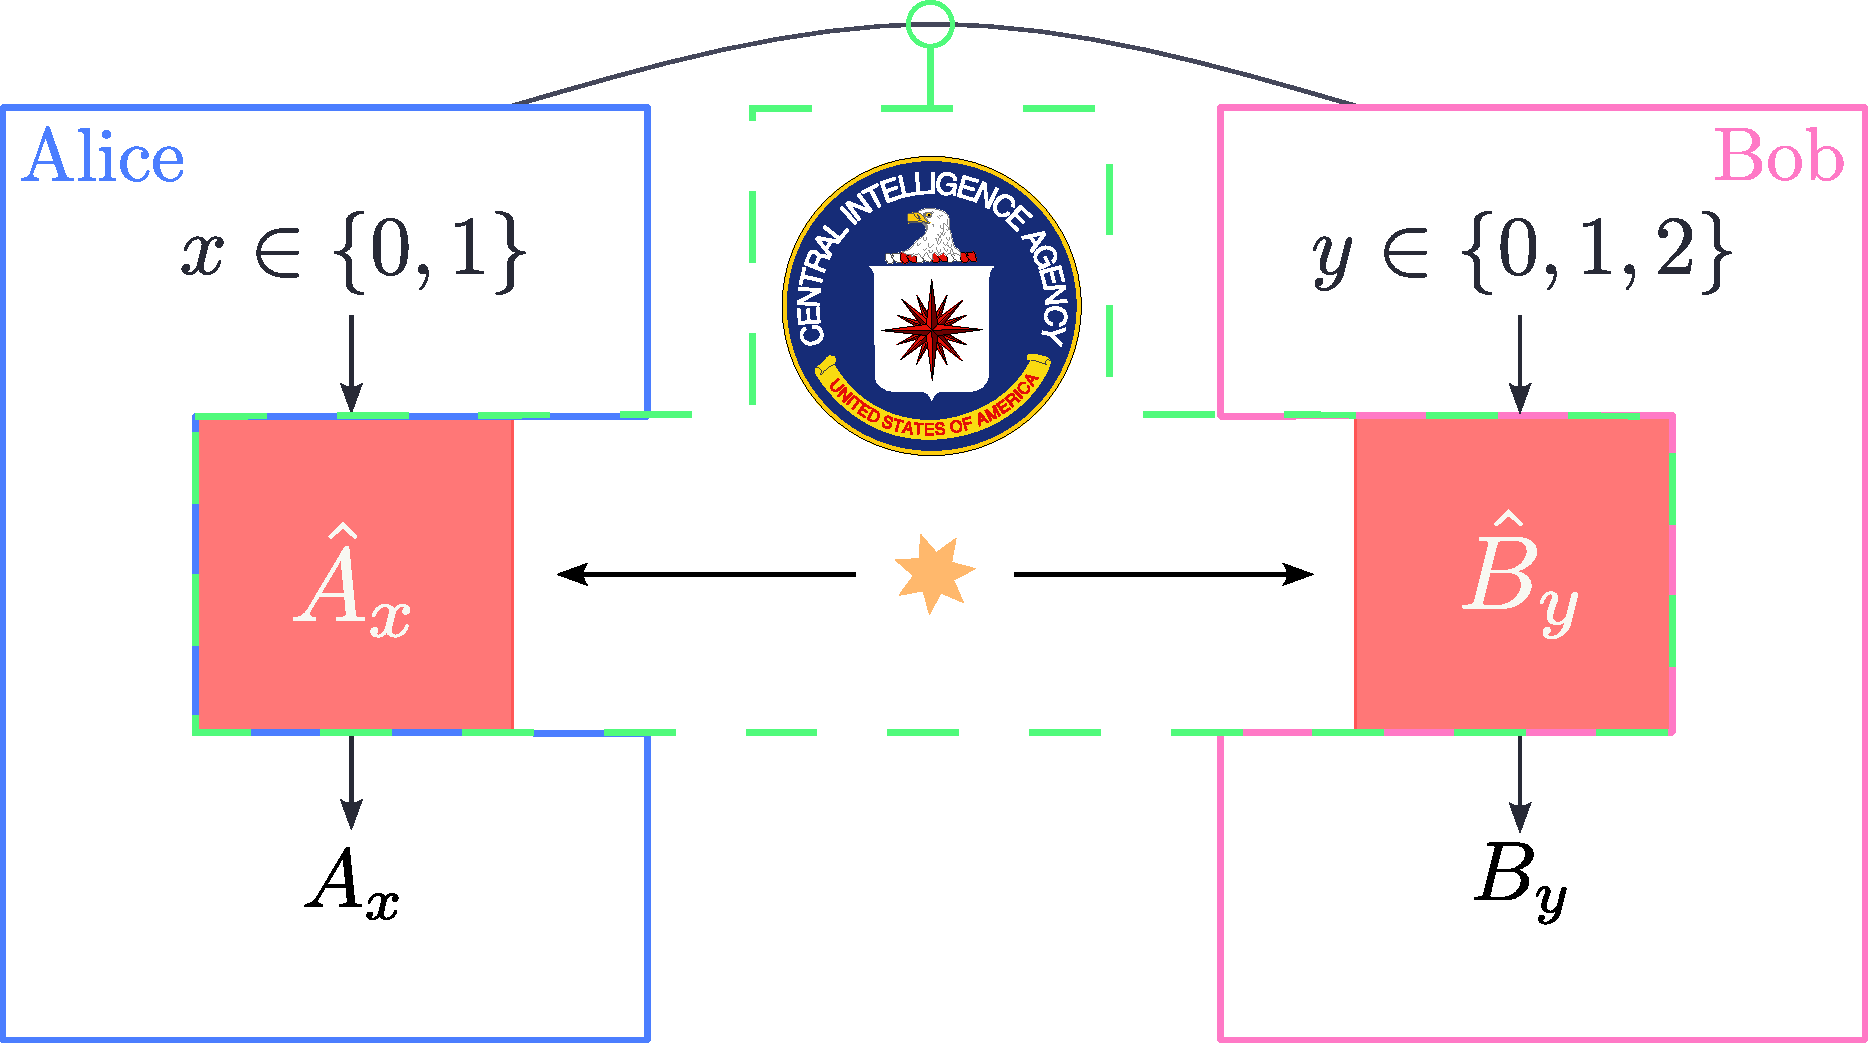
\includegraphics[width=0.95\textwidth]{chapters/deviceindependent/img/setup.pdf}
	\end{center}
	\caption{DIQKD Setup. Alice's lab (delimited by the blue line) and Bob's lab (delimited by the pink line) are linked by an authenticated classical channel of communication (gray craved line), and by a quantum channel (green dashed rectangle). A source (yellow star) generates a bipartite state with one part send to Alice while the other is send to Bob. Alice selects an input $x$, to perform the measurement $\hat{A}_x$ and obtain the outcome $A_x$. Similarly Bob chose an input $y$, to measure his
		received state with respect to $\hat{B}_y$ and obtain $B_y$.
	Eve, represented by the CIA logo, has full access on the quantum channel, the classical channel, and may have compromised the measurement devices. }
	\label{fig:DIQKD_setup}
\end{figure}

